\documentclass[12pt,answers]{exam}
\usepackage{amsmath}
\usepackage{lscape,multicol}
\usepackage[margin=1in]{geometry}
\usepackage{graphicx}
\usepackage{textcomp}
\usepackage{statex2}
\usepackage{shortvrb}
\usepackage{fancyhdr}
\MakeShortVerb{\!}
\usepackage{verbatim} % for comment environment

\begin{document}
\pagestyle{fancy}

\fancyhead[LH]{Ryan Gallagher}
\fancyhead[RH]{BIOS 04224 Exam 2}

\begin{questions}


\question Does RStudio support SAS?
\begin{solution}
No. RStudio does \textbf{not} support SAS.
\end{solution}


\question SAS is not free, but is it open-source software?
\begin{solution}
SAS is proprietary. \textbf{NOT} open source software.
\end{solution}

%\question Name 2 founders of SAS Inc.

\question
What is the name of the modern emacs mode which supports SAS and who
organized the free software project to create it?
\begin{solution}
Anthony Rossini created ESS(GPL) containing Emacs modes ESS[SAS], ESS[R], and ESS[Stata]. 
ESS[SAS] is the modern emacs mode which supports SAS.
\end{solution}

\question What is the most common SAS syntax error?
\begin{solution}
Forgetting the semi-colon to end a line is the most common SAS syntax error.
\end{solution}

\question After running a batch SAS program, what is the first thing
that you should do?
\begin{solution}
Check the .log file for errors!
\end{solution}

\question
\begin{parts}
\part When run in batch, are SAS programs compiled for speed
before execution? 
\begin{solution}
Yes. When run in batch, SAS programs is compiled \textbf{then} executed. This makes SAS very fast!
\end{solution}

\part Expand upon your answer above by contrasting the strengths and
weaknesses between R and SAS.
\begin{solution}
R is an interpreted language with an interpreter written in C and Fortran. Whereas SAS is a compiled language. Compiled languages are much faster than interpreted language because (in very basic terms) a compiled language is converted to machine code for the processor to execute, where an interpreted language need translation to machine language. Compiled languages are much faster than interpreted languages, but interpreted languages allow more flexibility and perhaps easier troubleshooting.
\end{solution}
\end{parts}

\question Which emacs/ESS keypresses do the following.

\begin{parts}
\part Refresh the current buffer.
\begin{solution}
F2 refreshes the current buffer.
\end{solution}
\part Save and submit a SAS program, the {\tt .sas} file, for batch processing.
\begin{solution}
F3 submits and saves the SAS program.
\end{solution}
\part Take you to the previously submitted SAS program from another buffer.
\begin{solution}
F4
\end{solution}
\part Load the SAS Log, the {\tt .log} file, refresh it, and take you to the first error, if any.
\begin{solution}
F5 loads the Log, refreshes it, and takes you to the first error. Also known as the .log file.
\end{solution}
\part Load the SAS Listing, the {\tt .lst} file, and refresh it.
\begin{solution}
F6 loads the SAS listing, or the .lst file, and refreshes it.
\end{solution}
\part Take you to the {\tt *shell*} buffer and create it if necessary.
\begin{solution}
F8 takes you to the {\tt *shell*} buffer.
\end{solution}
\part Load a permanent SAS data set of your choosing into {\tt PROC FSVIEW} for viewing.
\begin{solution}
F9 loads a permanent SAS data set into PROC FSVIEW for viewing. 
\end{solution}
\part Load a previously created SAS graphics stream file for viewing.
\begin{solution}
F12 loads a SAS graphics stream file for viewing.
\end{solution}
\end{parts}

\question What does ODS stand for and what is its purpose?
\begin{solution}
ODS stands for: \textbf{Output Delivery System}. It's main purpose is to capture SAS output in a data set for further processing and to  control the Statistics Graphics PROCs: SGPROCs
\end{solution}

\pagebreak

\question What is the ODS command to discover which analyses and
graphics figures will be produced by a given SAS procedure?
\begin{solution}
ODS TRACE statement writes to the SAS log a record of each output object that is created.
\end{solution}
\question Are ODS commands executed instantly or are they only
executed at the end of a block of code followed by a {\tt RUN;}
like all other SAS statements (besides {\tt RUN;} itself)?
\begin{solution}
ODS commands are executed instantly.
\end{solution}

\begin{comment}
\question How is the SAS macro facility like the C pre-processor, {\tt /bin/cpp}?
\begin{solution}
  Like {\tt cpp}, the SAS macro facility generates code that will be
  compiled and run.
\end{solution}

\question Which option is generally preferable for SAS macros and why: {\tt MPRINT} vs.\ {\tt NOMPRINT}?
\begin{solution}
{\tt MPRINT} is preferable.  It shows the SAS code that was generated
in the {\tt .log}
\end{solution}

\question What pre-existing software package does SAS/IML bear a suspicious resemblance to?
\begin{solution}
The Interactive Matrix Language (PROC IML) is remarkably similar
to S/R.
\end{solution}
\end{comment}
\hline
\textbf{For the SAS problems, I've included my thinking / rationale for each
question as comments in the .sas file.}\\
\hline
\question A common use of random sampling is when you have a large number
of subjects but it would be prohibitive to utilize all of them in your
study.  
\begin{parts}
  \part Suppose there are $N$ subjects and you want to randomly sample
  $n$.  Use SAS to randomly generate $N=25000$ values from the
  standard Uniform distribution, i.e., $z~\U{0, 1}$, and sample
  $n=500$ of them.  Don't forget to set your seed so that you can
  re-generate the same random stream in the future.
\begin{solution}
See prob11.sas \& prob11b.sas.
\end{solution}
\part Stratified random sampling divides all subjects into $M$ random
samples such that each sample is ``balanced'' with respect to one or
more strata.  For example, suppose that we want to draw a random
sample from the NTDB study preserving the distribution of GCSTOT in
each of the the $M$ samples. Create a SAS macro to perform stratified
random sampling and provide a random number seed for reproducibility.
\begin{solution}
See prob11.sas \& prob11b.sas \\  (prob11b.sas makes the macro, prob11.sas calls it)
\end{solution}
\end{parts}

\pagebreak 
\question Write a SAS macro to perform cold-decking.  Use the NTDB as
an example for the following variables: HISPANIC, MALE, SBP, PULSE and
RR.  Provide summaries before and after to demonstrate the degree
of missingness.  Also, demonstrate that the before and after
distributions are approximately the same via numerical summary (a
statistical test is not necessarily needed).

\begin{solution}
See prob12.sas. \\ \textbf{NOTE:} I had a lot of trouble with this problem. I couldn't figure out a way to do all variables at once, so I figured I could just do the single-variable cold-decking macro across all the required variables, then merge the data-sets. This worked for an arbitrary 25 observations, and still cannot for the life of me figure out why this macro doesn't work for more than 25 observation on the NTDB dataset. And what's worse, is I wasn't even getting error messages. Once I put (obs=26), the .sas would be stuck running forever and I would have to \texttt{kill \%1} - which yields no feedback. So currently I'm thinking either the gouda server was overloaded or something... and I was just not waiting long enough..? Either way, I wasn't able to check the if the distributions remained constant after my macro since the variables don't really have missing values at (obs=20). I still included the code I would've used to do this, but I wasn't actually able to check to see if it's true or not (although I don't know why it wouldn't be). 
\end{solution}

\question Write a SAS macro to generate a pallette of
colors from pure blue on one end of the spectrum to pure red on the
other and progressive mixtures of blue and red in between.  Hint see
the {\tt \%colormac} and {\tt \%helpclr} autocall SAS macros.

\begin{solution}
See prob13.sas. Below is the .png output.
\end{solution}

\begin{center}
\scalebox{1}{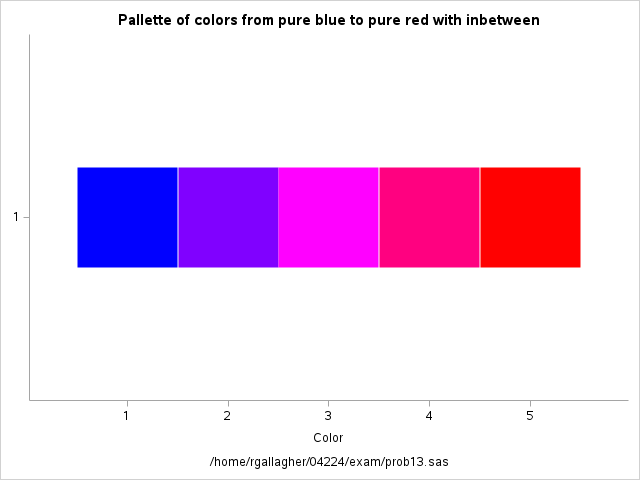
\includegraphics{prob13.png}}
\end{center}

\pagebreak

\question Based on Patel's 2x2 crossover trial data (you can find 
the data at \\
{\tt /data/shared/04224/latex/exam/crossover.sas}), do the following.
\begin{parts}
\part Summarize the mean values by group crossed with treatment period.
\begin{solution}
See crossover.sas. This is also preloaded in the crossover.lst file.
\end{solution}
\part Building upon these summaries, reproduce this figure with {\tt
  PROC SGPLOT}.
\begin{solution}
See crossover.sas. Below is the part (b) .png output.
\end{solution}
\begin{center}
\scalebox{1}{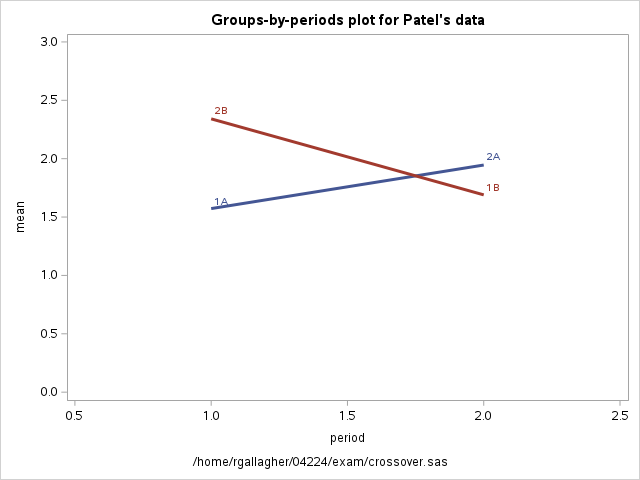
\includegraphics{crossover-b.png}}
\end{center}
\begin{center}
\scalebox{1.5}{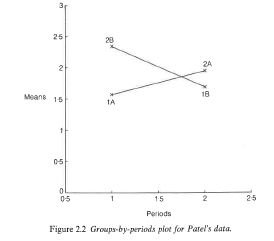
\includegraphics{figure-2-2.png}}
\end{center}
\pagebreak
\part With {\tt PROC SGPANEL} reproduce this figure.
\begin{solution}
See crossover.sas. Below is the part (c) .png output.
\end{solution}
\begin{center}
\scalebox{1.2}{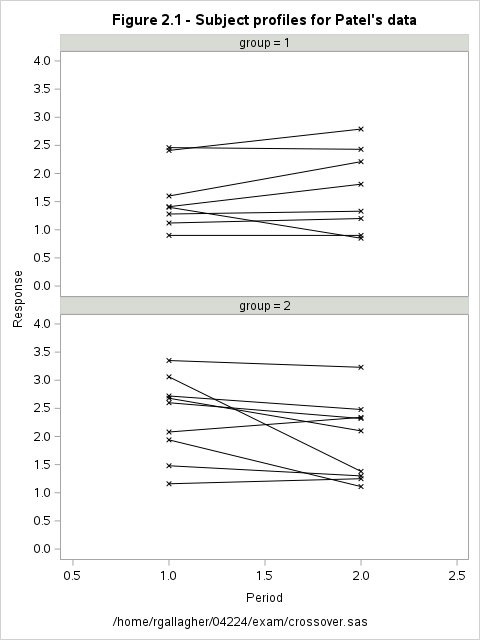
\includegraphics{crossover-c.png}}
\end{center}
\begin{center}
\scalebox{1.2}{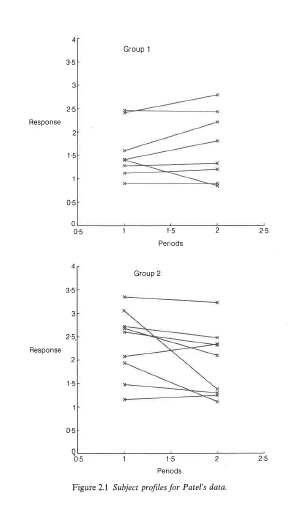
\includegraphics{figure-2-1.png}}
\end{center}
\pagebreak
\part
Jones and Kenward describe a graphical diagnostic technique for 2x2
crossover studies.  On the x-axis, plot the sum, $x=y_1+y_2$, vs.\ the
difference on the y-axis, $y=y_1-y_2$ (as seen below).  Overlay a
convex hull polygon around the two groups with {\tt SGPLOT} via
SGANNOTATE (hint: the {\tt SERIES} statement).
\begin{solution}
See crossover.sas Below is the part (d) .png output. \\ In /data/shared/04224/latex/exam, the file
`figure-2-3.pdf' is read-only, so I couldn't copy and include it in my .tex submission. 
\end{solution}
\begin{center}
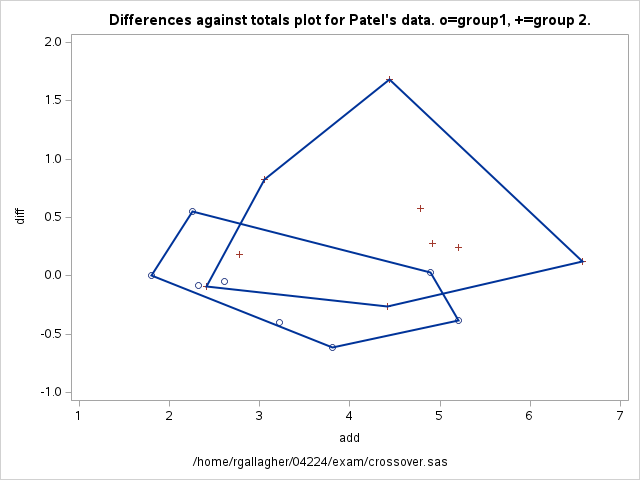
\includegraphics{crossover-d.png}
\end{center}
\end{parts}

\pagebreak

\question The US Census Bureau has divided the US into hierarchical
areas from the smallest, Census Blocks, up to Census Tracts, Counties,
States and Regions.  Typically, Census Blocks are areas that have
tangible boundaries like a city block (hence the name).  Data on
Census Blocks is not available to researchers due to the possibility
that subjects could be identified.  Census Blocks are accumulated into
Census Block Groups (CBG) for which the data is released.  And CBGs
are accumulated into Census Tracts.  Both CBGs and Census Tracts are
relatively homogeneous neighborhoods to reliably summarize.
\begin{parts}
\part
CBGs are used to derive the Area
Deprivation Index (ADI).  An ADI of 1 indicates the least deprived,
i.e., the best percentile.  An ADI of 100 indicates the most deprived,
i.e., the worst percentile.  However, the CRDW does not allow us to
have CBGs: the best we have is ZIP3 that is orders of magnitude
larger.  The ADI is not valid at the ZIP3 level (or any other level
besides CBG).  Therefore, make a map (of IL, MN and MI) where the
standard deviation of the subject's ADI is summarized.  The ADI
variable is ADI\_NARANK on F.US.  Does this map demonstrate that there
is a wide variability of ADI at the ZIP3 level?
\begin{solution}
See prob15.sas. Below is the part (A) .png output. This map shows that there is a very wide
variability in ADI per each ZIP3, especially since these values are on a scale of 1-100.
\end{solution}
\begin{center}
\scalebox{0.95}{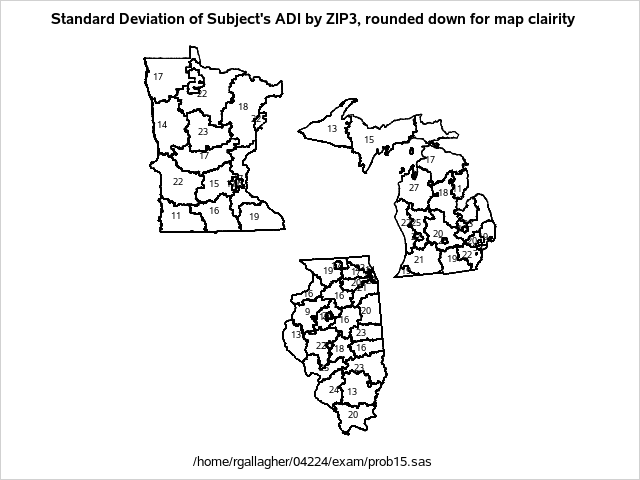
\includegraphics{prob15-1.png}}
\end{center}
\part Rural-Urban Commuting Area codes (RUCA) are defined
at the Census Tract level.  RUCA are integers 1 to 10: 1 for
metropolitan to 10 for rural area.  Make a map (of IL, MN and MI)
where the standard deviation of the subject's RUCA is summarized.  The
RUCA variable is SECONDARY\_RUCA\_CODE\_2010 on F.US.  Does this map
demonstrate that there is a wide variability of RUCA at the ZIP3
level?
\begin{solution}
See prob15.sas. Below is the part (B) .png output. This map demonstrates that there is indeed a variability of RUCA
at the ZIP3 level, but I think it's more reliable than ADI at the ZIP3 level (althought not by a whole lot since RUCA
is on a scale of 1-10). There is still information to be gained from this map since it shows the homogeniety of
'rural vs. urbal' among ZIP3s.
\end{solution}
\begin{center}
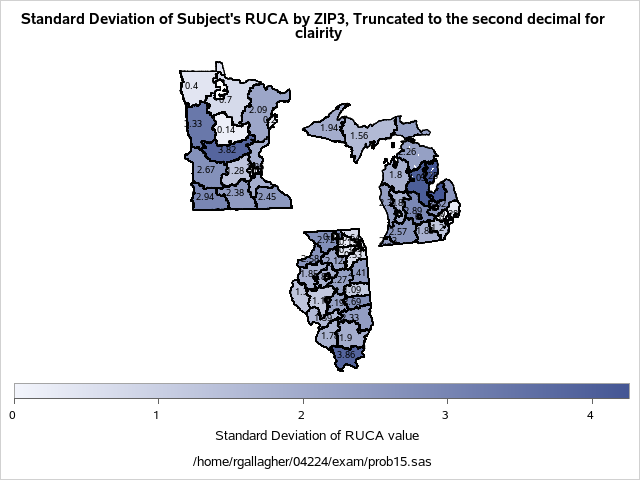
\includegraphics{prob15-2.png}
\end{center}
\end{parts}

\end{questions}

\pagebreak
\begin{center}
\section*{Some feedback for this course}
\end{center}

Firstly I'd like to thank you, Professor Rodney, for your time teaching this course and the resources you created for future use of R, SAS, Linux, Emacs, etc.. Those slides I will assuredly be downloading and kept for future reference. One of the huge draws to me as a Master's student was the technical education I'd be gaining as someone who would like to persue a career in data science, data analytics, or statistics generally. While job searching before starting my studies at MCW, most listings required experience in SAS/R so I'm very greatful to say I now have real experience using these tools.
\\


I do believe there was a lot of value in learning Linux/Emacs with these languages. You mentioned that you believe it'd be difficult for someone to jump into the R half or SAS half of this course, and I agree. However, I think SAS has more reliance on EMAC/Linux than R, so perhaps SAS+Linux+Emacs would be necessary, but I think R could be taught without. 
\\


A suggestion I have for integrating LaTeX (more) into this course could be to require assignments be submitted using it. I feel LaTeX is really intuitive, and I think if you required student to use it that they'd figure it out and learn something along the way. This is how I learned it in my undergraduate Abstract Algebra course, at least.
\\

Finally, I'd like to express my difficulty with the partner homework structure. I do believe it works well in theory and for grading purposes, however, my experience had me doing an assignment solo and submitting it with mine and someone elses name on it. My partner clearly struggled with this class's content, but in order to keep my grade up it meant submitting assignments in this paired homework structure. And just to be clear -- as someone who really saw the value in learning SAS/R, I didn't mind doing the assignments for my own education, but I just don't think the homework grade associated with my partner's is accurately relective of his effort/knowledge of the course topics.
\\

Again, thank you for your time and efforts instructing this programming course. I really did get a lot out of it, and I think it'll go a long way with where I want my future career to be. 
\\
\\
\\
-Ryan
\end{document}

